\documentclass{article}

% if you need to pass options to natbib, use, e.g.:
%     \PassOptionsToPackage{numbers, compress}{natbib}
% before loading neurips_2019

% ready for submission
% \usepackage{neurips_2019}

% to compile a preprint version, e.g., for submission to arXiv, add add the
% [preprint] option:
%     \usepackage[preprint]{neurips_2019}

% to compile a camera-ready version, add the [final] option, e.g.:
     \usepackage[final]{neurips_2019}

% to avoid loading the natbib package, add option nonatbib:
%     \usepackage[nonatbib]{neurips_2019}

\usepackage[utf8]{inputenc} % allow utf-8 input
\usepackage[T1]{fontenc}    % use 8-bit T1 fonts
\usepackage{hyperref}       % hyperlinks
\usepackage{url}            % simple URL typesetting
\usepackage{booktabs}       % professional-quality tables
\usepackage{amsfonts}       % blackboard math symbols
\usepackage{nicefrac}       % compact symbols for 1/2, etc.
\usepackage{microtype}      % microtypography
\usepackage{graphicx}
\usepackage[english]{babel}
\usepackage{caption}
\usepackage[style=numeric, defernumbers, backend=biber]{biblatex}
\usepackage[labelfont=bf]{caption}
\addbibresource{library.bib}

\title{Multimedia retrieval}




\date{June 2021}

\begin{document}

\maketitle
\begin{abstract}
TBD


 
\end{abstract}


%===== SECTION =====
\section{General Introduction (draft)}
The overall objective of the project is the following: Build a content-based 3D shape retrieval system that, given a 3D shape, finds and shows to the user the most similar shapes in a given 3D shape database. To reach this, a pipeline has to be created consisting of various components that, among other things, process, extract and evaluate shapes and shape data. 

The report comprises three main segments containing various sub-tasks, that are executed sequentially and aim to achieve the aforementioned goals. The first two sections will cover the loading, pre-processing and cleaning of the data. The following two sections entail the main underlying mechanisms that allow an end-user to query by example and for the system, in turn, to retrieve similar shapes. The final two steps aim to assess and improve the built system in terms of scalability and evaluation metrics.

[[Insert MR pipeline picture]]

\section{Read and view the data}

% STRUCTURE DRAFT 
\subsection{Description and goal}
The goal of this step is to, not only, become familiar with several building blocks for the project, like the shapes database itself, but also build a tool that can load and view them. The tool also has to adhere to various shape visualization requirements and functionalities.

\subsection{Shapes database and element notation}
The shapes database contains hundreds of 3D mesh files of different types and classes, however each shape has several spatial data properties which will be defined in the following table and used throughout subsequent sections.

\begin{center}
\begin{table}[h]
    \centering
    \begin{tabular}{c|c|c}
    \hline
         \textbf{Name} & \textbf{Notation} & \textbf{Expression} \\
         \hline
         Vertex & $v_i$, V & $v \in V$ \\
         \hline
         Edge & $e_i$, E & $\{v_i, v_j\} \subseteq E$ \\
         \hline
         Face & F & $\{e_1, e_2...e_n\} \subseteq E $ \\  
         \hline
         Cell & c_i & $(p_i, p_{i+1})$ \\
         \hline
         Basis function & $\phi_i$ & $\phi_i(x)$ \\
         \hline
         Mesh & M & $(V, E, F)$ \\
         \hline
         Wireframe & W & $(V, E)$ \\
         Placeholder & ... & ... \\
         \hline
         Placeholder & ... & ... \\
         & 
    \end{tabular}
    \caption{Caption}
    \label{tab:my_label}

\end{table}
\end{center}

\newpage
\subsection{Execution}
The tool that was built uses extensive python libraries for user interface and for loading the shapes. These are: Vedo [ref] for shapes loading, processing and PyQT5 [ref] for UI window rendering.

When opening the tool one can first select a category or class of shapes and then a specific shape to be viewed. As required, one can also switch display types of the shape. These are:
\begin{itemize}
    \item Shaded
    \item Wireframe
    \item Wireframe over shaded
\end{itemize}
The following functionalities are also implemented:
\begin{itemize}
    \item Rotate viewpoint around shape
    \item Zoom in/out
    \item Pan (translate)
\end{itemize}

See figures 1-3 for a demonstration of these requirements.
\begin{figure}[h]
    \centering
    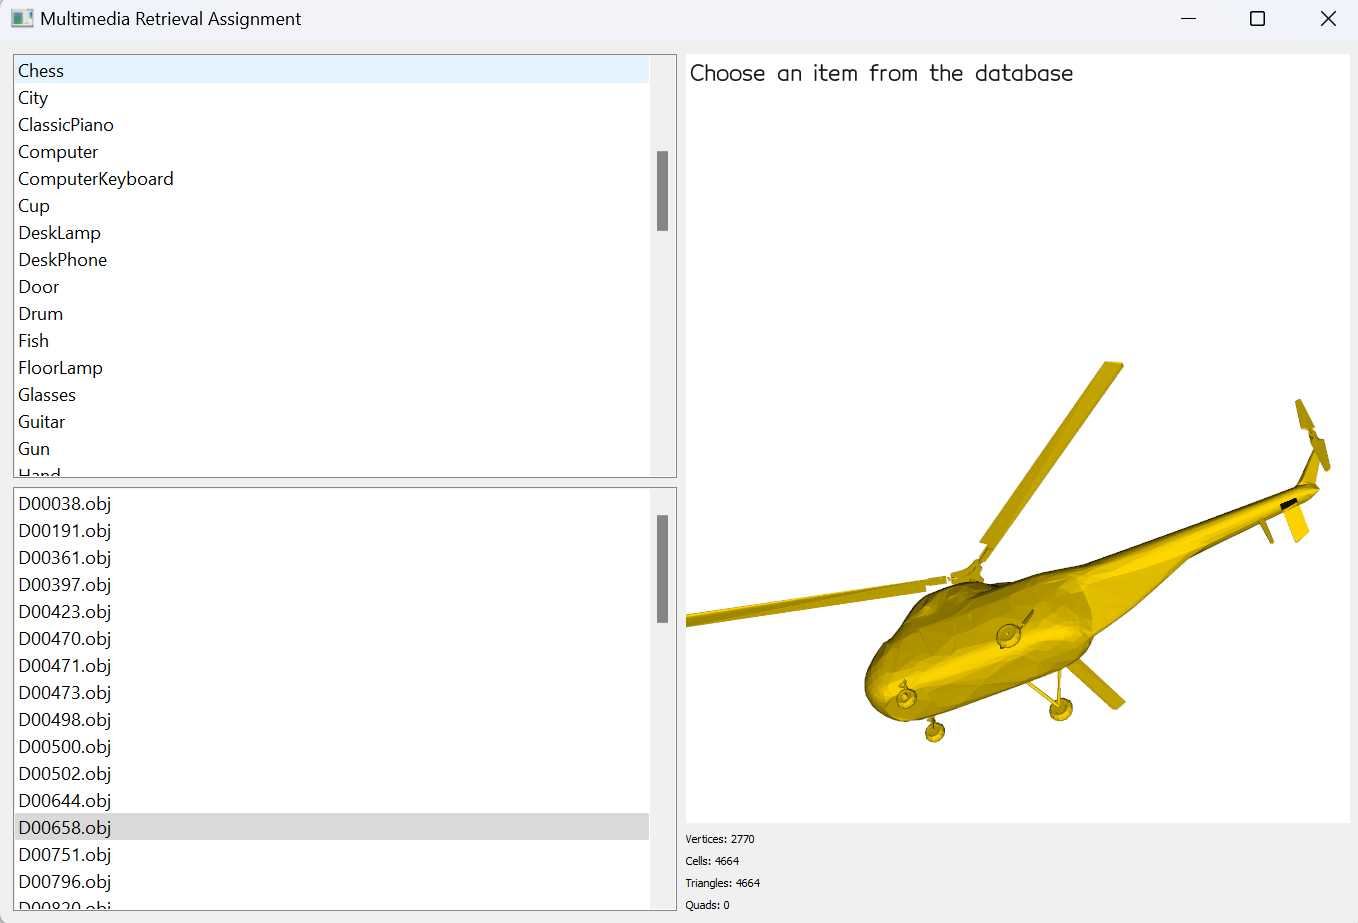
\includegraphics[scale=0.3]{example_pan_rotate.png}
    \caption{Application example where object mesh ($M$) is panned and rotated}
\end{figure}

\begin{figure}[h]
    \centering
    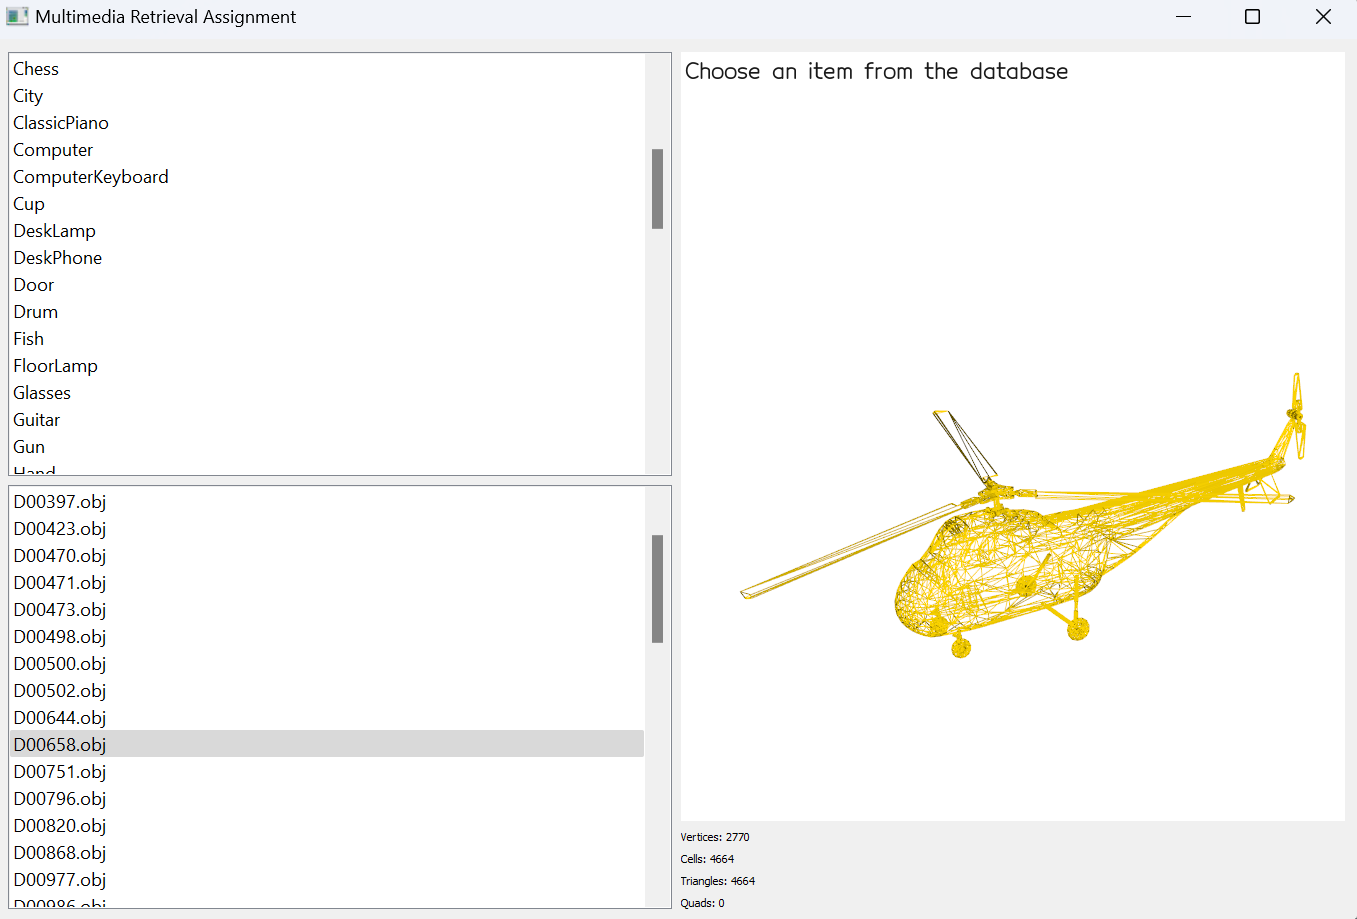
\includegraphics[scale=0.3]{example_wireframe.png}
    \caption{Application example where a wireframe ($W$) is generated}
\end{figure}

\newpage
\subsection{Testing}
The library was tested with shapes of different varieties and polygons. Even with shapes that contain many vertices like that of a shrub, there were no issues found. 

\medskip

\small


\printbibliography



\end{document}